\documentclass[CS4402-Notes.tex]{subfiles}
\begin{document}

\section{Modelling}

\subsection{Abstract constraint models}
Constraint modelling is often considered the step to map a well-defined problem statement in a constraint language into a solver-independent constraint model for a constraint solver to solve and find solutions to. Solvers like Savile Row can take a solver-independent model and convert it into its own solver-specific model. However, when viewing constraint models \textit{abstractly}, it can be seen that many combinatorial problems that we wish to tackle exhibit some \textit{common features}.
\n
Many problems require the programmer to find objects such as:
\begin{itemize}
\item (Multi-)sets
\item Relations
\item Functions
\end{itemize}
The abstract constraint model can be written in terms of there patterns. However, the patterns are typically not supported directly by constraint solvers (unlike intensional constraints. As such, the pattens need to be modelled as constrained collections of more primitive objects.
\begin{figure}[H]
\centering
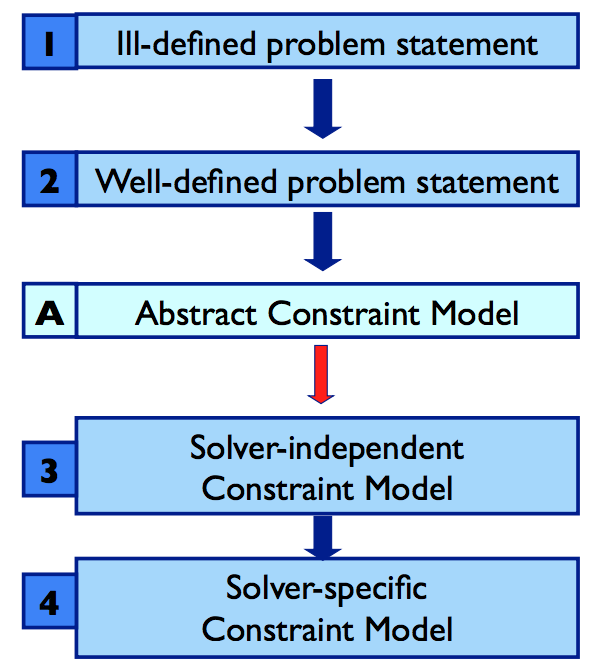
\includegraphics[width=0.5\textwidth, keepaspectratio]{imgs/modelling-steps.png}
\caption{Steps to model a problem for a particular constraint solver.}
\end{figure}
\noindent
This way, the corresponding \textbf{modelling patterns} for representing and constraining these combinatorial objects can be developed and effort is reduced when modelling new problems. Writing abstract constraint models gives a much richer set of types of decision variables, such as sequences, sets and functions and allows the programmer to extract the common features and patterns among different problems. Constraints for these variables and the objective function can also use operators on these new types of objects, such as set union, set relation etc. Finally, the patterns can be combined to model more compex problems.

\subsection{Sequences}
A sequence is defined as an \textbf{ordered list of elements}. It simply has elements in order and repetition is allowed. In the simple case, a sequence in of \textbf{fixed length}, or is \textbf{bounded} by a maximum length. The trickiest case for sequences is when the length is \textbf{unbounded}. Unbounded sequences are a problem because solvers need to use a finite-domain to model the CSP. In these cases, the programmer must be smart to find a bound by reading the problem carefully.
\begin{itemize}
\item 0, 1, 1, 2, 3, 5, 8, 14
\item Turn right, drive 1 mile, turn right, drive 0.5 miles, turn left
\end{itemize}
are examples of sequences. This pattern typically occurs in planning problems, where a sequence of actions is the solution to transform the initial state of the problem into a goal state. Other examples include Langford's problem and the Bombastic problem.

\subsubsection{Fixed-length sequences}
Fixed-length sequences are problems of the form:
\begin{itemize}
\item Given \textbf{n}
\item Find a sequence of objects of length \textbf{n}
\item Such that ...
\end{itemize}
For example the magic sequence problem (CSPLib 19):
\begin{itemize}
\item Given \textbf{n}
\item Find a sequence \textbf{S} of integers $s_{0}, ..., s_{n}$
\item Such that there are $s_{i}$ occurrences of $i$ in \textbf{S} for each $i$ in $0, ..., n$.
\end{itemize}
For the problem instance $n = 9$, a possible solution would be $6, 2, 1, 0, 0, 0, 1 , 0, 0, 0$
\n
To model fixed-length sequences, the most straightforward model is to use an array of decision variables indexied $1...n$ where the domains are the objects to be found.
\begin{figure}[H]
\centering
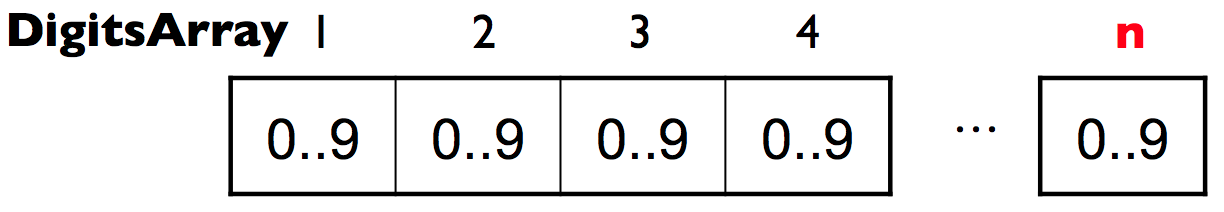
\includegraphics[width=0.8\textwidth, keepaspectratio]{imgs/digits-array.png}
\caption{Array of decision variables 1 to n with their domain specified in an array.}
\end{figure}
\noindent
As a constraint, this can be written as follows:
\begin{lstlisting}
  Forall i in 0..n .
      No. of occurences of i in S of i is S[i]
\end{lstlisting}
Depending on the constraint language being used, this statement may need to be expressed more or less concisely. For example, Essence Prime has a constraint \texttt{gcc(X, Vals, C)} which states that for each non-decision expression \texttt{Vals[i]}, the number of occurrences of \texttt{Vals[i]} in \texttt{X} equals \texttt{C[i]}.
\begin{lstlisting}[caption={The Magic Sequence problem modelled in Essence Prime.}]
  language ESSENCE' 1.0

  given n : int
  find x: matrix indexed by [int(0..n)] of int(0..n)

  such that
  gcc(x, [i | i : int(0..n)], x)
\end{lstlisting}
\begin{itemize}
\item \texttt{x} is the array whose values we are counting and is represented by a matrix of decision variables
\item \texttt{[i | i : int(0..n)]} is the list of values to count, which is a matrix of non-decision variables. The syntax here is a comprehension to produce the values \texttt{[0,1...,n]}
\item \texttt{x} is used a second time here as the number of occurrences of each value, as it is the same as the value that is being counted
\end{itemize}

\subsubsection{Bounded-length sequences}
Bounded-length sequences are similar to fixed-length sequences, except that the length cannot exceed the maximum. The problems come in the form:
\begin{itemize}
\item Given \textbf{n}
\item Find a sequence of objects of length \textbf{at most n}
\item Such that ...
\end{itemize}
The Kiselman Semigroup Problem (KSP) is an example of a problem with infinite domain, but can be bound to a maximum length depending on the problem instance. The problem states that:
\begin{itemize}
\item Given $n$, a positive integer
\item Find a sequence of integers drawn from $1..n$
\item Such that between every pair of occurrences of an integer $i$, there exists an integer greater than $i$ and an integer less than $i$
\end{itemize}
An example solution for $n = 3$ would be $2, 3, 1, 2$. In the definition of this problem, it can be seen that it is not finite. To \textit{Find a sequence of integers drawn from $1..n$}, the sequence can be infinitely long. This is a problem because we want to map the abstract constraint model down to a finite-domain CSP and this is not possible with an infinite domain in the abstract model. To deal with this, we must derive a finite domain for KSP. Notice that there can be at most 1 occurences of 1 and $n$. Likewise:
\begin{itemize}
\item At most 2 occurences of 2 and $n - 1$
\item At most 4 occurences of 3 and $n - 2$
\end{itemize}
From this pattern, we can derive a maximum sequence length of $\sum^{n}2^{n/2} - 1$ pairs, which gives a finite domain for the sequence variable. Finally, because we have set a maximum length to the sequence, we may have to use \textbf{dummy variables} in solutions that are less than the maximum length, but still valid solutions.
\n
We have to be careful when using dummy variables, especially if the value of the dummy exists in the domain of the variables as this will create \textbf{equivalence classes} of assignments. In that case it is impossible to tell if the value assigned to the variable is a real value or a dummy value. The solution to deal with this is to choose a \textbf{canonical element} from each class. For example, saying all 0s must appear at the end of the sequence if the dummy value is 0. Then the constraint will make sure to reject all other equivalences. Introducing equivalances during modelling is something that happens very often and one must be aware of this happening to use appropriate measures to counter it.

\subsubsection{Unbounded sequences}
For some problems, the issue of infinite domains cannot be dealt with in a smart way. This usually happens when a bound cannot be derived, or the derived bound is too weak to be useful. Problems with infinite domains are common when modelling planning problems, for example how many steps are needed to evacuate the building? Or how many actions it neeeded to reach the goal state?
\n
Though inefficient, the solution to this is to solve a series of CSPs by incrementally increasing the length of the sequence. Moreover, this method allows the solver to find a solution with the shortest possible sequence.

\subsubsection{Permutations}
Some problems involve finding a sequence of elements where:
\begin{itemize}
\item The elements in the sequence are known
\item The arrangement of elements is not known
\end{itemize}
The goal is then to find a \textbf{permutation} of the sequence that satisfies the constraints. The Travelling Salesman Problem (TSP) is an example of finding permutations, as the network between the cities and distances are all known.

\subsubsection{Viewpoints}
A \textbf{Viewpoint} is a choice of variables and domains sufficient to characterise the problem. In other words, if there is an assignment to the chosen variables, it can be read off a solution to the problem. Note this doesn't say anything about constraints.
\n
For example, when looking for permutations, we can explore two different viewpoints:
\begin{enumerate}
\item Assume that the elements of the permutation are distinct. This leads to a fixed-length viewpoint.
  \begin{figure}[H]
  \centering
  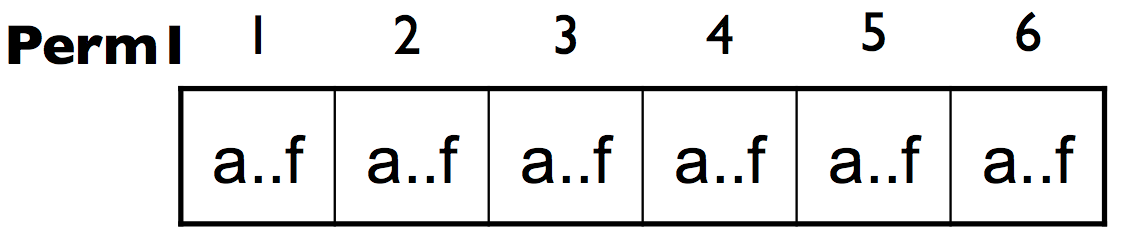
\includegraphics[width=0.6\textwidth, keepaspectratio]{imgs/perm1.png}
  \caption{First viewpoint for a permutation which contains elements $a, ..., f$}
  \end{figure}
\item Alternatively, we know the elements appear in the sequence, so we can index by those elements. The domain values now represent the position in the sequence an element is in.
  \begin{figure}[H]
  \centering
  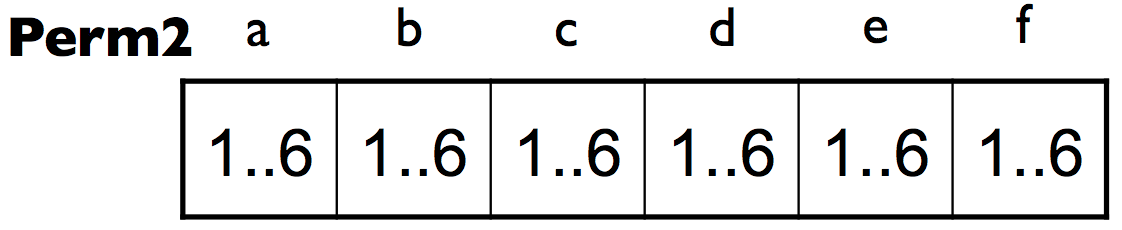
\includegraphics[width=0.6\textwidth, keepaspectratio]{imgs/perm2.png}
  \caption{Second viewpoint for a permutation, using indices instead of elements.}
  \end{figure}
\end{enumerate}
Now there are two different viewpoints to choose from and this will depend on the kind of constraints needed to find a solution. For example, if the constraint is \textit{a and b must be adjacent}, then the second viewpoint it much easier to model with the constraint \texttt{| Perm2[a] - Perm2[b] | = 1}. On the other hand, if the constraint is \textit{The first three letters of the sequence must form an English word}, then it is easier to model the constraitn using the first viewpoint.

\subsection{Sets}
A set is a collection of \textit{distinct} objects not arranged in any particular order. The items in a set must be unique (no duplicates). Examples of set would be $\{1, 2, 3\}$ or \{red, green, blue\}.

\subsubsection{Fixed-cardinality sets}
Consider the following simple problem class:
\begin{itemize}
\item Given $n$ and $s$
\item Find a set of $n$ digits that sum to $s$
\end{itemize}
There are two ways to represent this problem, the \textbf{explicit representation} and \textbf{occurence representation}.

\subsubsection{Explicit representation}
For the explicit representation, an array $E$ is introduces to hold the decision variables indexed by $1..n$, each with a domain of $0..9$. The constraint for the problem is then simply:
\begin{lstlisting}
  AllDifferent(E)
  Sum(E) = s
\end{lstlisting}
However, the issue of equivalence classes once again comes up here. The two sets \{1,3,5,7\} and \{7,3,5,1\} are equivalent as the order does not matter in a set, so a way to deal with this equivalence must be introduced.
\begin{table}[H]
\centering
\begin{tabular}{| c | c | c | c |}
\hline
\textbf{1} & \textbf{2} & \textbf{3} & \textbf{4} \\
\hline
1 & 3 & 5 & 7 \\
\hline
\end{tabular}
\caption{Explicit array representation of the set \{1,3,5,7\}}
\vspace{1cm}
\begin{tabular}{| c | c | c | c |}
\hline
\textbf{1} & \textbf{2} & \textbf{3} & \textbf{4} \\
\hline
7 & 3 & 5 & 1 \\
\hline
\end{tabular}
\caption{Equivalent array reprensentation of the set \{7,3,5,1\}}
\end{table}
A simple way to doing this would be to use ascending order as the canonial element from each class. Then the \texttt{AllDifferent(E)} constraint will be replaced by \texttt{E[1] < E[2] < E[3] < E[4]}.

\subsubsection{Occurrence representation}
Another way to represent sets is with an occurrence representation. This never introduces equivalence classes. It works like an array of binary switches. Following the above example, an occurrence representation $O$ would be an array of 0/1 decision variables indexed by $0..9$:
\begin{table}[H]
\centering
\begin{tabular}{| c | c | c | c | c | c | c | c | c | c |}
\hline
\textbf{0} & \textbf{1} & \textbf{2} & \textbf{3} & \textbf{4} & \textbf{5} & \textbf{6} & \textbf{7} & \textbf{8} & \textbf{9} \\
\hline
0,1 &  0,1 & 0,1 & 0,1 & 0,1 & 0,1 & 0,1 & 0,1 & 0,1 & 0,1 \\
\hline
\end{tabular}
\end{table}
Now we simply need the two constraints:
\begin{lstlisting}
  sum(O) = n
  O[1] + 2O[2] + 3O[3] + ... + 9O[9] = s
\end{lstlisting}
The first constraint only allows $n$ 1s to be filled in the occurrence array and the second constraint is the constraint for the sum of digits.
\n
Both explicit representation and occurrence representation have their advantages and disadvantages. For some problems, an explicit representation may introduce equivalence classes and be more complicated to specify a constraint. For example, if we wanted to say \textit{if 5 is in the set, then so is 4}, this would need a constraint that takes more computation in the explicit representation.
\begin{figure}[H]
\begin{minipage}{0.42\textwidth}
\begin{lstlisting}[caption={Explicit representation}]
Forall j in 1..n .
    If (E[j] = 5)
        Exists i in 1..j-1 . E[i] = 4
\end{lstlisting}
\end{minipage}
\hspace*{\fill}
\begin{minipage}{0.42\textwidth}
\begin{lstlisting}[caption={Occurrence representation}]
(O[5] = 1) -> (O[4] = 1)
\end{lstlisting}
\end{minipage}
\end{figure}
\noindent
It should be noted that a combination of explicit and occurrence representations can be used to model problems, for example the intersection of two occurrence representations is an explicit representation. In other words, the two are not mutually exclusive. Obviously, constraints on the original sets have to be modelled appropriately.

\subsubsection{Set constraints}
As sets appear frequently in constraint problems, it is useful to look at how common constraints such as intersection, union and subset are modelled. Any complex constraint can be decomposed to a simple constraint, each of which has at most one operator and possible one equality sign. For example, the complex constraint
\begin{equation}
(A \cup B) \subseteq (C \cap D)
\end{equation}
can be decomposed into three constraints
\begin{align}
  X &= A \cup B \\
  Y &= C \cap D \\
  X &\subseteq Y
\end{align}

\subsubsection{Set intersection}
The set intersection constraint can be modelled with both the explicit and occurrence representations. Take the simple constraint $A \cap B = C$ where $A$ and $B$ are sets of digits (domain 0..9), an occurrence representation would model it as the following three arrays
\begin{figure}[H]
\centering
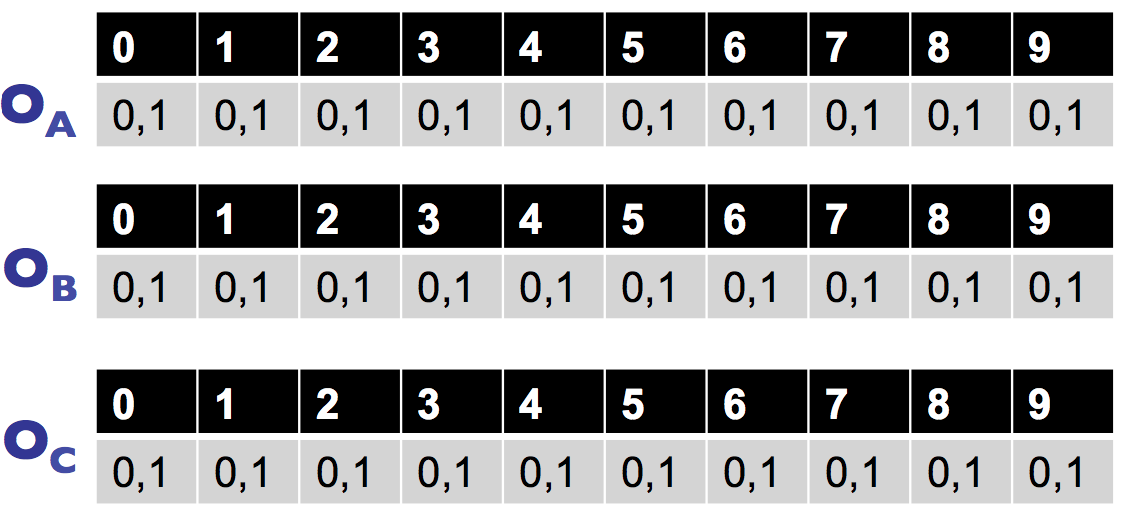
\includegraphics[width=0.7\textwidth, keepaspectratio]{imgs/intersection-occurrence.png}
\caption{Three arrays of switches that map to $A, B$ and $C$.}
\end{figure}
\noindent
with the constraint
\begin{lstlisting}
  Forall i in 0..9 .
    O$_{\texttt{C}}$[i] = O$_{\texttt{A}}$[i] $\times$ O$_{\texttt{B}}$[i] 
\end{lstlisting}
To use explicit representation here would be more complicated and require more complex constraints.
\begin{figure}[H]
\centering
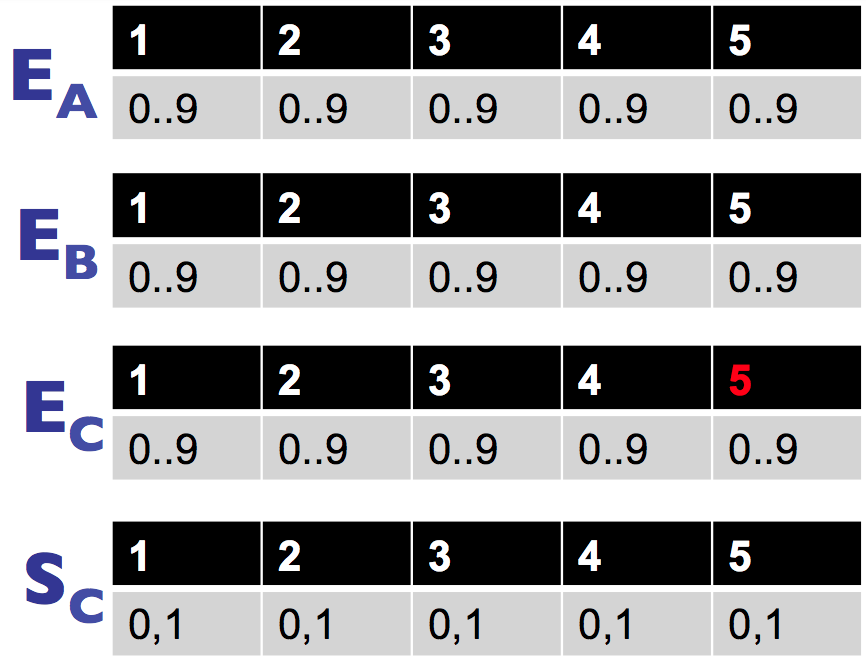
\includegraphics[width=0.6\textwidth, keepaspectratio]{imgs/intersect-explicit.png}
\caption{Arrays for explicit representation of set intersection. Cardinality of 5.}
\end{figure}
\noindent
Each array represents the 5 values in the sets $A, B, C$, but the constraint to expresss the intersection is more complicated. Furthermore, it requires an extra marker array \texttt{S$_{\texttt{C}}$}.
\begin{lstlisting}
  Forall d in 0..9 .
    Forall i in 1..5 .
      If (E$_{\texttt{A}}$[i] = E$_{\texttt{B}}$[i]) && (E$_{\texttt{B}}$[i] = d) . 
        d must appear in E$_{\texttt{C}}$[i]
\end{lstlisting}

\subsubsection{Set union}
The same arrays as in set intersection can be used to model the set union $A \cup B  = C$ simply with a different constraint for an occurrence representation.
\begin{lstlisting}
Forall i in 0..9 . 
  O$_{\texttt{C}}$[i] = (O$_{\texttt{A}}$[i] = 1 $\vee$ O$_{\texttt{B}}$[i] = 1)
\end{lstlisting}
Again this will be more complicated using an explicit representation which will be omitted here.

\subsubsection{Set subset}

\subsection{Multisets}
A multiset (sometimes referred to as ``bags'') is like a set except that duplicate values \textit{are} allowed. They are also not arranged in any particular order and are typically characterised by the number of times each obejct occurs in the multiset. The multiset pattern occurs in places like the packing problem, for example a bag with a number of coloured balls.
\n
Like sets, we must bound the domain of a multiset to be finite. For example,
\begin{itemize}
\item Let $S$ be a finite set of size $n$.
\item The domain ``set of $S$'' comprises of every set whose elements are members of $S$. This domain is the \textbf{power set} of $S$ with size $2^{n}$.
\item The domain ``multiset of $S$'' will comprise of every finite multiset whose elements are all members of $S$. This will have an infinite domain as long as $S$ is non-empty due to infinite repetition.
\end{itemize}
To ensure that the multiset of $S$ is finite, we must bound either the total number of elements in the multiset, or bound the number of occurrences of each value.

\subsubsection{Explicit representation}


\subsubsection{Occurrence representation}
In the occurrence representation of multisets, instead of using 0 or 1 as values in the array, the array is extended to allow multiple occurrences.

\subsection{Relations}
Relations are an assignment of truth values to tuples of values. For example, in the set $P = \{\text{Bill}, \text{Bert}, \text{Tom}\}$, a binary relation \textit{like} can be defined between two people from the set $P$. The cross product $P \times P$ can be used to get all tuples of the set $P$. We might assign the tuple $<$Bill, Bert$>$ and $<$Bert, Tom$>$ to be true and false for all other combinations. To visualise an occurrence representation of a relation $R$ between two sets, a table can be created.
\begin{figure}[H]
\centering
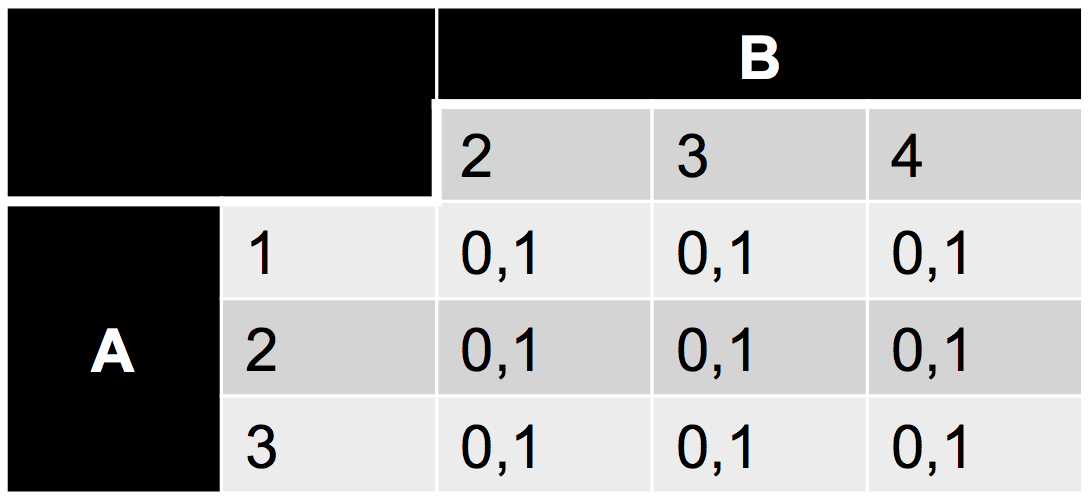
\includegraphics[width=0.4\textwidth, keepaspectratio]{imgs/relation-occurrence.png}
\caption{Occurrence relation between two sets $A = \{1,2,3\}$ and $B = \{2,3,4\}$}
\end{figure}
\noindent

\subsubsection{Projection}
A common operation on relations in a projection. A relation can be projected onto one or more of its arguments, which results in a relation of reduced arity (less arguments/operands). For example in the set $P = \{\text{Bill}, \text{Bert}, \text{Tom}\}$ with the relation \textit{likes} on $P \times P = \{<\text{Bill, Bert}>, <\text{Bert, Tom}>, <\text{Bert, Bill}>\}$, the projection of \textit{likes} onto Bert gives $\{\text{Tom, Bill}\}$.

\subsubsection{Other representations}
From simple binary relations, relations can be extended to k-ary relations. This is best thought of using a k-dimensional matrix. For exmaple in the ternary case of $A \times B \times C$, we can introduce a 3D matrix indexed by elements of $A$ and $B$ and the size of $C$.

\subsection{Functions}
A function $f$ is a binary relation on two sets: a domain and a \textbf{codomain} (aka range). It has the property that each element of the domain is related to at most one element of the range which can be written as $f(x) = y$ to mean that the image of $x$ under the function $f$ is $y$.
\begin{figure}[H]
\centering
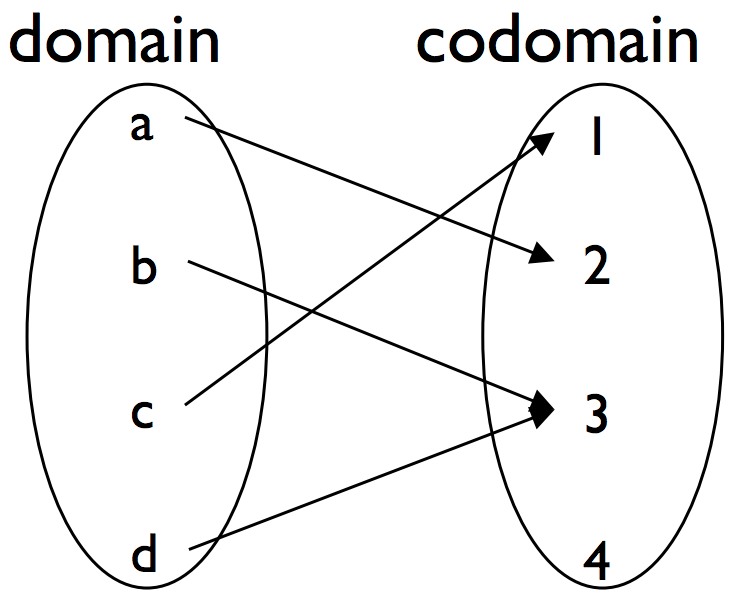
\includegraphics[width=0.3\textwidth, keepaspectratio]{imgs/function.png}
\end{figure}
\noindent
In a \textbf{total} function, every element of the domain has an image in the codomain while in a \textbf{partial} function, some elements have no image in the codomain. For an explicit representation of partial functions, dummy elements have to be introduced, preferrably outside of the range of codomain values to avoid equivalence classes.

\subsubsection{Injections}
The images of two distinct elements of the domain under an \textbf{injective} function are distinct. In other words, no two domain values map to the same codomain value. An \texttt{AllDifferent} constraint will need to be added for these cases.
\n
A \textbf{partial injection} is more complicated as not all domain values have to be mapped, but mapped values must be distinct.
\begin{figure}[H]
\centering
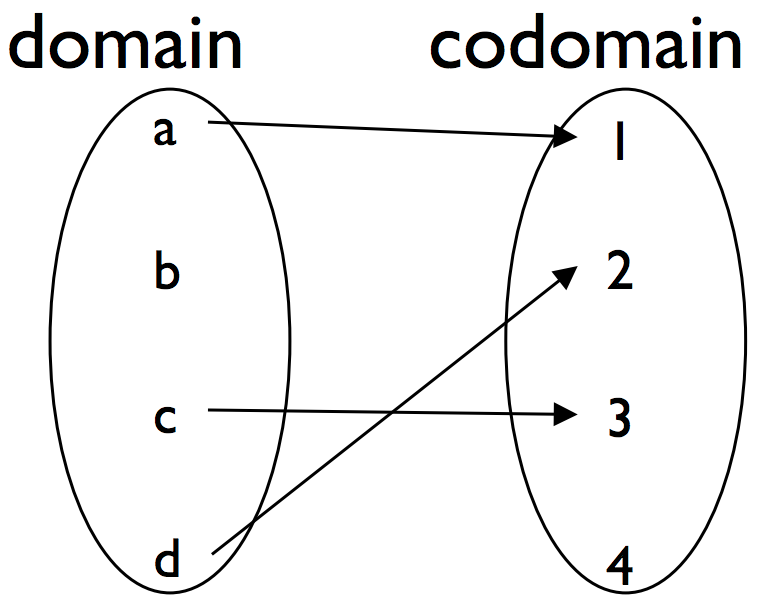
\includegraphics[width=0.3\textwidth, keepaspectratio]{imgs/partial-injective-function.png}
\caption{Domain and codomain mapping for partial injective functions.}
\end{figure}
\noindent
Using an explicit model is messier here, but the occurrence representation is easy as we need the constraint that the sum of each row and col are both $\leq 1$.
\n
Furthermore, there are \textbf{surjective} functions, where every element of the codomain must be mapped to some element of the domain and \textbf{bijections}, which is both an injection and surjection. 


\subsection{Nested structures}
Though we have explored many methods to model combinatorial objects, problems often require us to find one combinatorial objected nested inside another, for example a set of sets or a sequence of functions.

\subsubsection{The Gripper Problem}
In the gripper problem, the robot must move the 4 balls from room A to room B. The goal is to have all balls in room B and the robot has three actions: pick up, put down and move.
\begin{figure}[H]
\centering
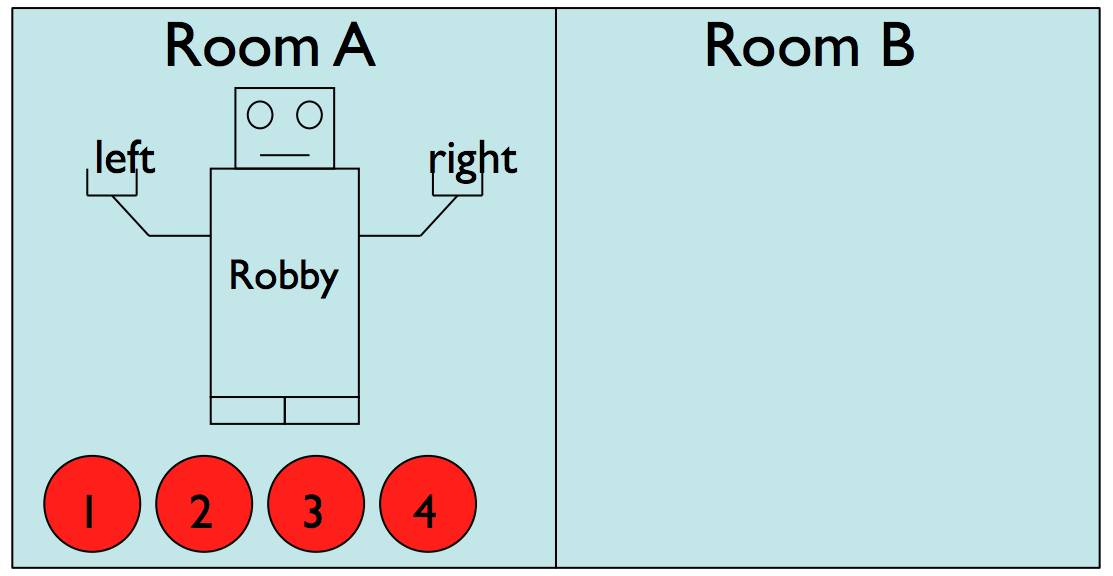
\includegraphics[width=0.7\textwidth, keepaspectratio]{imgs/gripper-problem.png}
\end{figure}
\noindent
Since the robot has two hands, it can pick up or put down two balls in a single step. However, when he moves, he can't pick up or put down balls when he is moving. Hence there are at most 2 actions per step. Naturally, this is characterised as a \textbf{sequence of sets} with a maximum cardinality of 2.

\subsubsection{Nesting inside sequences}
Recall how fixed-length sequences of size $n$ can be represented as an array of decision variables indexed from $1..n$ where the domains are the objects to be found.
\begin{table}[H]
\centering
\begin{tabular}{| c | c | c | c | c | c |}
\hline
\textbf{0} & \textbf{1} & \textbf{2} & \textbf{3} & \textbf{...} & \textbf{n} \\
\hline
0..9 & 0..9 & 0..9 & 0..9 & ...& 0..9 \\ 
\hline
\end{tabular}
\end{table}
In the case of nested sequences, we can no longer use a single variable at each index to represent the object at that position because one variable is not enough to represent our set, function or relation. A simple solution is to extend the dimension of the array. By having more dimensions, we can now have a column of variables for each index to represent the nested structure.

\subsubsection{Nesting inside sets}
Nested structures inside sets is being asked to find a set of some other object. Both the model of the outer type and model of the inner type (explicit/occurence) must be specified here, unlike in the case of nested sequences, where only one type was needed.
\n
Consider the following problem class:
\begin{itemize}
\item Given $m, n$
\item Find a cardinality-$m$ set of sets of $n$ digits such that ...
\item There are three possibilities for models:
  \begin{enumerate}
  \item An occurrence representation
  \item Outer: Explicit. Inner: Occurrence
  \item Outer: Explicit. Inner: Explicit
  \end{enumerate}
\end{itemize}
\textbf{Nested sets: occurrence representation} \\
It is not feasible to introduce an occurence array indexed by the possible set of $n$ digits as this is not scalable. The size of the array would need to encompasss every possible set of size $n$ digits which would be too large.
\begin{table}[H]
\centering
\begin{tabular}{| c | c | c | c |}
\hline
\textbf{\{1, 2, 3\}} & \textbf{\{1, 2, 4\}} & \textbf{\{1, 2, 5\}} & ... \\
\hline
0,1 & 0,1 & 0,1 & ... \\ 
\hline
\end{tabular}
\end{table}
Because of this, nested outer layers are typically represented explicitly.
\n
\textbf{Nested sets: Outer explicit} \\
To express the outer layer explicitly, the dimension of the explicit array can be extended according to the representation chosen from the inner set. Of course, we have to be careful to make sure the elements of the outer set are distinct.

\begin{figure}[H]
\centering
\begin{subfigure}{0.45\textwidth}
\centering
\begin{tabular}{| c | c | c | c | c |}
  \hline
  \textbf{EO} & \textbf{1} & \textbf{2} & \textbf{...} & \textbf{m} \\
  \hline
  \textbf{0} & 0,1 & 0,1 &  & 0,1 \\
  \hline
  \textbf{1} & 0,1 & 0,1 &  & 0,1 \\
  \hline
  \textbf{...} & & & & \\
  \hline
  \textbf{9} & 0,1 & 0,1 &  & 0,1 \\
  \hline
\end{tabular}
\caption{Occurrence representation of inner set}
\end{subfigure}
%
\begin{subfigure}{0.45\textwidth}
\centering
\begin{tabular}{| c | c | c | c | c |}
  \hline
  \textbf{EE} & \textbf{1} & \textbf{2} & \textbf{...} & \textbf{m} \\
  \hline
  \textbf{1} & 0..9 & 0..9 &  & 0..9 \\
  \hline
  \textbf{2} & 0..9 & 0..9 &  & 0..9 \\
  \hline
  \textbf{...} & & & & \\
  \hline
  \textbf{n} & 0..9 & 0..9 &  & 0..9 \\
  \hline
\end{tabular}
\caption{Explicit representation of inner set}
\end{subfigure}
\end{figure}

\begin{figure}[H]
\centering
\begin{subfigure}{0.45\textwidth}
\begin{lstlisting}[caption={Constraints for occurrence representation of inner set}]
Forall i in 1..m . 
  sum(col i of EO) = n

Forall i in 1..m-1 .
  col i of EO < col i+1 of EO
\end{lstlisting}
\end{subfigure}
\hspace*{\fill}
\begin{subfigure}{0.45\textwidth}
\begin{lstlisting}[caption={Constraints for occurrence representation of inner set}]
  AllDiff on each column
    
  Forall i in 1..m-1 .
    col i of EE < col i+1 of EE
\end{lstlisting}
\end{subfigure}
\end{figure}

\subsubsection{Relations as sets of tuples}
Previously, we viewed relations as an assignment of truth values to tuples of values. This can be represented as a set of tuples.

\subsection{Symmetry}
The concept of symmetry is a \textbf{structure-preserving transformation} which can be characterised as a bijection on assignments (i.e. a one-to-one mapping). Complete assignments are partitioned into equivalence classes where all members in every class is either a solution or no member is a solution. In other words, symmetry preserves solutions. If there is a solution, symmetrical instances will also have solutions and vice versa.
\n
In constraint programming, we do not want to deal with symmetries as it can lead to a lot of wasted effort for systematic search. There are two common special cases of symmetry:
\begin{enumerate}
\item Variable symmetry - where the bijection can be characterised in terms of variables alone
\item Value symmetry - where the bijection can be characterised in terms of values alone
\end{enumerate}

\subsubsection{Variable symmetry}
Variable symmetry can be expressed in terms of a bijection on the variables. For example in the 4-queens problem, the board can be flipped horizontally, which leads to another valid and symmetrical solution.
\begin{figure}[H]
  \centering
  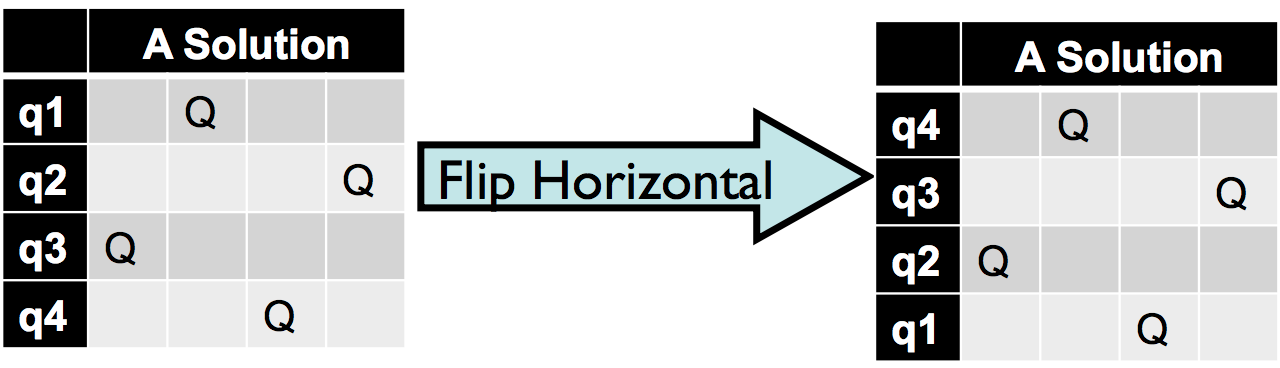
\includegraphics[width=0.9\textwidth, keepaspectratio]{imgs/4-queens-symmetry.png}
  \caption{Two symmetrical solutions to the four queens problem.}
\end{figure}
\begin{itemize}
\item q1 $\rightarrow$ q4
\item q2 $\rightarrow$ q3
\item q3 $\rightarrow$ q2
\item q4 $\rightarrow$ q1
\end{itemize}
A bijection of values would capture the transformation of this particular solution - but not the general horizontal flip. Equivalently, a symmetrical non-valid solution is still non-valid.

\subsubsection{Value symmetry}
In value symmetry, the values assigned to variables can be permuted to give a symmetrical solution. An example of this is the graph colouring problem.
\begin{figure}[H]
\begin{subfigure}{0.42\textwidth}
  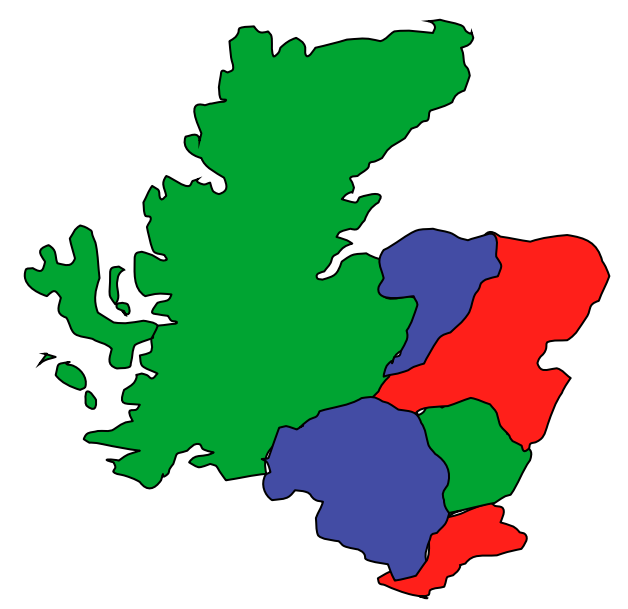
\includegraphics[width=1\textwidth, keepaspectratio]{imgs/map-colouring1.png}
  \caption{Solution to graph colouring problem with map of Scotland.}
\end{subfigure}
\hspace*{\fill}
\begin{subfigure}{0.42\textwidth}
  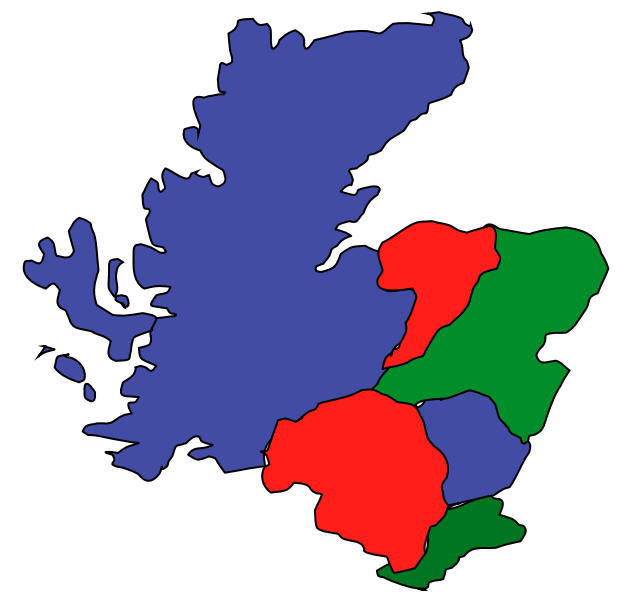
\includegraphics[width=1\textwidth, keepaspectratio]{imgs/map-colouring2.png}
  \caption{Symmetrical solution by permuting the value of the colours.}
\end{subfigure}
\label{fig:graph-colouring}
\end{figure}
\noindent
A symmetrical solution can be reached as shown in figure \ref{fig:graph-colouring} by permuting the colours as follows:
\begin{itemize}
\item red $\rightarrow$ green
\item green $\rightarrow$ blue
\item blue $\rightarrow$ red
\end{itemize}

\subsubsection{Consequences of symmetry}
Assuming that an explored subtree contained no solutions, symmetries in the model can map this fruitless subtree into another. If the symmetry is not dealt with, a systematic search will explore all symmetric variants of this subtree. It is important to remember symmetrical non-solutions are also non-solutions, and this is much more common than symmetrical solutions.
\begin{figure}[H]
  \centering
  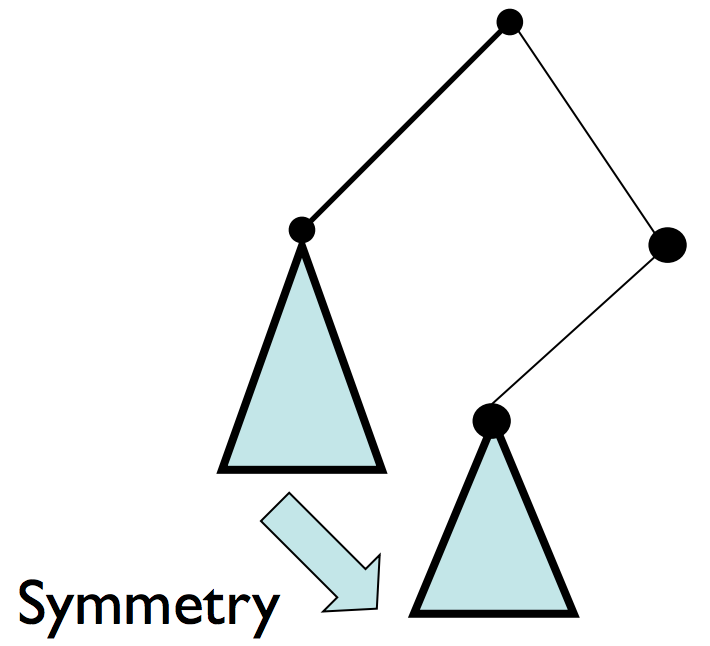
\includegraphics[width=0.4\textwidth, keepaspectratio]{imgs/symmetrical-subtree.png}
  \caption{Symmetrical subtrees can map to another subtree later in the search.}
\end{figure}

\subsubsection{Symmetry-breaking constraints}
Knowing how symmetry is introduced during modelling can make some symmetry detection easy. There are two reasons that symmetry enters into a constraint model:
\begin{enumerate}
\item It is inherent in the problem by nature, for example in the n-queens problem as the solution is a square
\item It is introduced during the modelling process, especially for explicit representations.
\end{enumerate}
Adding constraints can affect the symmetry, for example by disallowing some elements of an equivalence class of assignments. This is typically done by defining an ordering of elements. Ordering the elements distinguishes one element in each equivalence clas of assignments. If the symmetry-breaking constraint is effectively propagated, the search tree can be pruned drastically. Valid symmetry-breaking constraints leave at least one element in each equivalence class of assignments, so they throw away solutions to the original problem. This is fine as we can recover those solutions by applying the symmetry to the solutions allowed. Moreover, if enough symmetry-breaking constraints are added, \textit{all} symmetry can be broken.
\n
Typically, symmetry-breaking constraints are formulated by defining a canonical solution and adding constraints to choose it. In other words an ordering on variables and an order on solutions is needed.

\subsubsection{Lex-leader method}
To define an ordering, it is often best to use a \textbf{lexicographic} ordering, for example
\begin{equation}
\{a, b, c, d\} \leq_{\text{lex}} \{b, d, c, a\}
\end{equation}
The lex-leader method is a way of applying lexicographic ordering to break all symmetry at the cost of a large number of constraints needed. It does so in two simple steps:
\begin{enumerate}
\item Choose an ordering on the variables
\item Add one lexicographic orderin constraint per symmetry
\end{enumerate}
Although a huge number of constraints might be needed, sometimes the lex constraints collapse into simpler forms (like in the explicit set representation). The compromise is to only use a subset of the lex-leader constraints. For example, given the array
\begin{table}[H]
\centering
\begin{tabular}{| c | c | c |}
  \hline
  A & B & C \\
  \hline
  D & E & F \\
  \hline
\end{tabular}
\end{table}
with row and column symmetry, an ordering on variables ABCDEF can be chosen. With the lex-leader method, the following constraints have to be defined for the various types of symmetry that exist.
\begin{itemize}
\item ABCDEF $\leq_{\text{lex}}$ DEFABC - Swapping rows
\item ABCDEF $\leq_{\text{lex}}$ ACBDFE - Swapping last two columns
\item ABCDEF $\leq_{\text{lex}}$ DFEACB - Swapping rows and last 2 columns
\item ...
\end{itemize}
This prevents it from being possible to obtain a ``smaller'' assignment that the one currently defined by applying symmetry. Depending on the problem, this could require a factorial number of constraints, which is too many and unscalable. This is where the $\text{Lex}^{2}$ ordering comes in.

\subsubsection{$\text{Lex}^{2}$ ordering}
A significant fraction of the lex-leader constraints for row/column symmetry can be represented by lex ordering only the rows and columns.

\subsection{Viewpoints}
The fundamental formulation to any constraint model is the selection of a viewpoint. A viewpoint is defined as a set of decision variables and domains sufficient to characterise the problem. The rest of the model and constraints follows from this choice of variables and domains.
\n
Selecting a good viewpoint is essential to constraint modelling as a wrong choice can be writing the constraints very awkward, which likely leads to poor solver behaviour. Additionally, a good viewpoints makes expressing some of the constraints easier, but maybe not all constraints, so one viewpoint can be saved and auxiliary variables used to express the remaining constraints.

\subsubsection{Auxiliary variables}
Each variable in a CSP represents a choice that must be made to solve the problem being modelled. Because the original viewpoint is sufficient to represent all choices in the original problem, these \textbf{auxiliary variables} are extra in the sense that they are not needed to characterise the problem. In other words, the axuiliary variables are separate from the viewpoint that express constraints not in terms of the variables in the viewpoint.
\n
As the choices that the auxiliary variables represent must also be represented by the original viewpoint, we must ensure that the two sets of variables are consistent by introducing \textbf{channelling constraints}.
\begin{figure}[H]
\centering
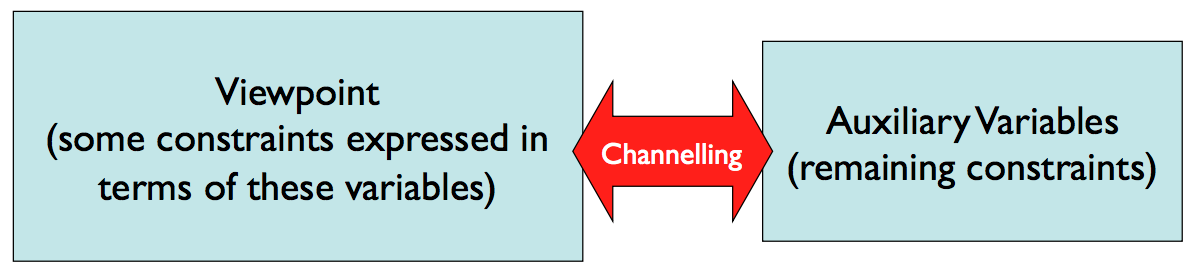
\includegraphics[width=0.8\textwidth]{imgs/channelling-constraints.png}
\caption{Auxiliary variables connected with channelling constraints to the original viewpoint.}
\end{figure}
\noindent
Sometimes it is useful to formulate a model with 2 or more viewpoints to more easily express certain constraints. To add channelling constraints to link the auxiliary variables and original viewpoint, often a variable in one viewpoint has to be mapped or related in some way to the variables in the other viewpoint. Sometimes, extensional constraints work better here than intensional constraints.

\subsection{Branching variables}
Given a viewpoint and axuiliary variables, it is usually not necessary to assign all the variables to get a solution, as they may be redundant. The subset of the variable we choose to search over are the \textbf{branching} variables. It must be ensured that assigning the selected branching variables is sufficient to produce a solution. This is a choice that is made, especially when there are two viewpoints. The criteria for choosing which variables is to try and maximise constraint propagation.

\subsection{Implied constraints}
Implied constraints are logical consequences of the initial specification problem, when there is a chain of reasoning that leads to a deduction of implied constraints from the initial constraints. It is important to note that in theory, if constraint propagation was powerful enough, the solver would be able to see all these logical consequences, however, this is not the case in practice.
\n
The constraints programmer must add implied constraints explicitly, to help reduce the amount of search needed in the solver. This needs to be done by hand because the generation of implied constraints involves complex reasoning steps which are difficult to automate. Further, programmers have to learn to do this by experience, as it is often the case implied constraints are missed because it logically does not need to be written explicitly.
\n
There is a difference here between implied constraints and \textbf{redundant} constraints. The latter is also implied by the initial problem specification, but does not reduce search. These constraints should be avoided when possible as they add overhead to the solver and slow down the solving process.
\n
Finally, symmetry-breaking constraints are \textit{not} implied, as the CSP obtained by breaking-symmetry is not equivalent to the original problem in that it has a different set of solutions. In fact, when we break symmetry, there are new implied constraints that can be inferred. Often, the most powerful implied constraints are derived from symmetry-breaking, because more information can be inferred about the problem and therefore a stronger implied constraint can be written. For example, in the \texttt{AllDifferent} constraint on the explicit representation of sets
\begin{table}[H]
\centering
\begin{tabular}{| c | c | c | c | c |}
  \hline
  \textbf{1} & \textbf{2} & \textbf{3} & ... & \textbf{n} \\
  \hline
  0..9 & 0..9 & 0..9 & ... & 0..9 \\
  \hline
\end{tabular}
\end{table}
the symmetry-breaking constraint
\begin{equation*}
  E[1] \leq  E[2] \leq E[3] \leq ... \leq E[n]
\end{equation*}
introduces a new implied constraint
\begin{equation*}
E[1] < E[2] < E[3] < ... < E[n]
\end{equation*}
making the original \texttt{AllDifferent} constraint redundant. 
\end{document}

